Nessa etapa nosso objetivo é cálcular a distribuição de velocidades e 
das componentes e demonstrar esta segue distribuição de Maxwell-Boltzman (\ref{eq:distr-maxwell-boltzmann1}, \ref{eq:distr-maxwell-boltzmann2}, \ref{eq:distr-maxwell-boltzmann3})
\begin{align}
    P(v) &\sim \frac{v^2}{K_B T} \exp \left( - \frac{m v^2}{2K_B T} \right) \label{eq:distr-maxwell-boltzmann1}  \\ 
    P(v_x) &\sim \frac{1}{\sqrt{K_B T}}\exp \left( - \frac{m v_x^2}{2K_B T}  \label{eq:distr-maxwell-boltzmann2}\right)\\
    P(v_y) &\sim \frac{1}{\sqrt{K_B T}}\exp \left( - \frac{m v_y^2}{2K_B T}  \label{eq:distr-maxwell-boltzmann3}\right)
\end{align}

Para isso foi utilizado o código do item anterior(\ref{ssec:codigoA}),  com algumas adições para computar a magnitude da velocidade após atingir equilíbrio (depois de 1000 iterações). 
Então foram obtidos os dados para intervalos de $t=20$ à $40$ e assim por diante. E nessa simulação 
consideramos os pontos para iterações de multiplos de $20 \Delta t$. 
Na figura(\ref{fig:distribuicoes-velocidade-b})
podemos ver os histogramas criados para magnitude e as componentes da velocidade assim como 
a curva teórica das distribuições de Maxwell-Boltzmann. 

\begin{figure}[h!]
    \centering
    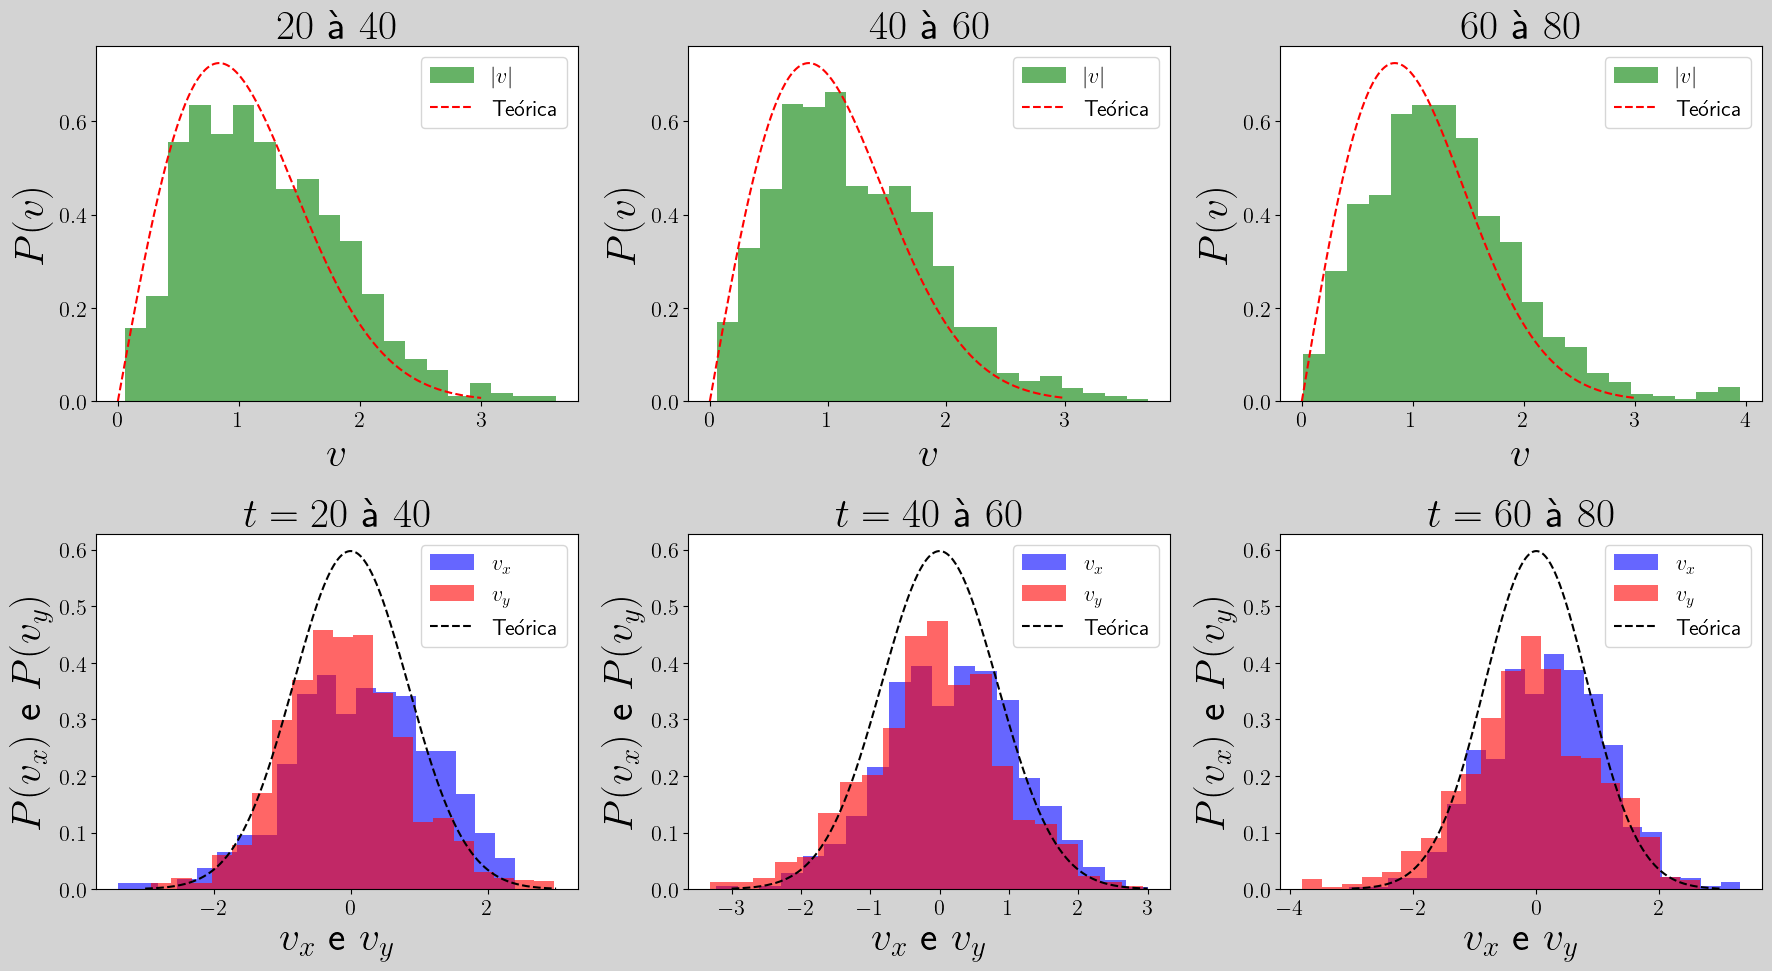
\includegraphics[width=0.7\linewidth]{tarefa-B/distribuicoes-b.png}
    \caption{Distribuição da velocidade, magnitude e componentes em intervalos $t=20-40$, $t=40-60$ e $t=60-80$.}
    \label{fig:distribuicoes-velocidade-b}
\end{figure}

Esse é o comportamento antecipado para o sistema, já que para essa simualação iniciamos as partículas em uma 
malha regular, embora com algum deslocamento aleatório, e iniciamos todas elas com velocidades de igual magnitude e só 
componentes aleatórias. Após muitas iterações o esperado é que o sistema se estabilize com velocidades médias muito 
parecidas para as partículas. Entretando ainda obtivemos flutuações nas distribuições de velocidade. Isso pode 
se dar ao fato de estarmos considerando apenas a cada $2 \Delta t$.\footnote{Combinado às flutuações já discutidas das condições periódicas de contorno.}

No próximo item estudamos as mesmas distribuições, porém considerando perfis de velocidade 
iniciais diferentes. 

Além do calculo das distribuições nessa etapa também foi gerado um \verb|gif| com animação da dinâmica. 
Encontra-se em \verb|graficos/tarefa-B/evolucao.gif|. 

\clearpage